\bivtask{Drehung um eine Gerade durch den Nullpunkt}{10}
%
Gegeben sei ein Richtungsvektor $v = \pmat{a \\ b \\ c} \in ℝ^3$,
$\|v\|_2 = 1$, und ein Winkel $\theta$. Bestimmen Sie die
Transformationsmatrix für die Drehung um den Winkel $\theta$ um die
Gerade, die durch den Ursprung in Richtung von $v$ verläuft.

\begin{center}
  \begin{picture}(0,0)%
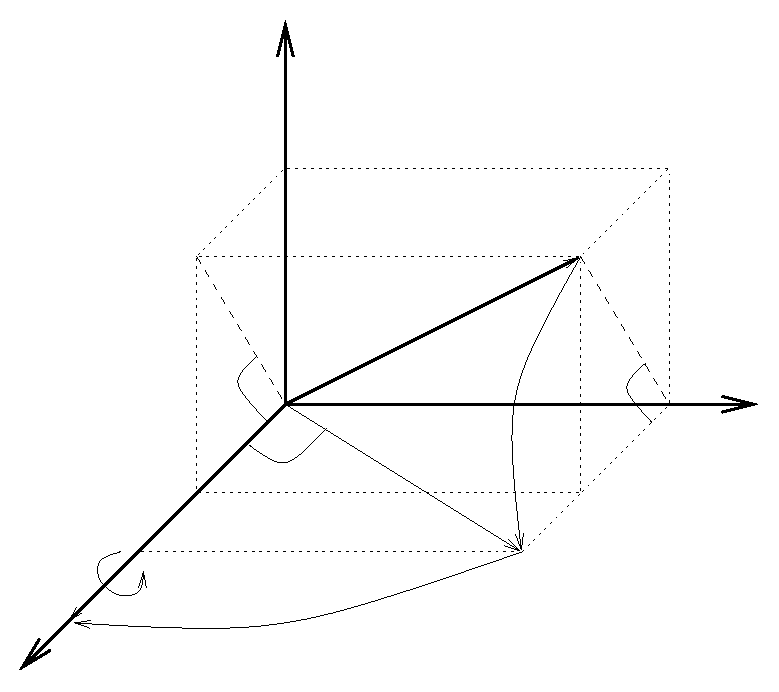
\includegraphics{drehung3D}%
\end{picture}%
\setlength{\unitlength}{4144sp}%
%
\begingroup\makeatletter\ifx\SetFigFont\undefined%
\gdef\SetFigFont#1#2#3#4#5{%
  \reset@font\fontsize{#1}{#2pt}%
  \fontfamily{#3}\fontseries{#4}\fontshape{#5}%
  \selectfont}%
\fi\endgroup%
\begin{picture}(5669,5012)(654,-4376)
\put(2836,479){\makebox(0,0)[lb]{\smash{\SetFigFont{10}{12.0}{\familydefault}{\mddefault}{\updefault}{\color[rgb]{0,0,0}$y$}%
}}}
\put(6256,-2221){\makebox(0,0)[lb]{\smash{\SetFigFont{10}{12.0}{\familydefault}{\mddefault}{\updefault}{\color[rgb]{0,0,0}$x$}%
}}}
\put(5041,-1321){\makebox(0,0)[lb]{\smash{\SetFigFont{10}{12.0}{\familydefault}{\mddefault}{\updefault}{\color[rgb]{0,0,0}$v$}%
}}}
\put(5626,-2491){\makebox(0,0)[lb]{\smash{\SetFigFont{10}{12.0}{\familydefault}{\mddefault}{\updefault}{\color[rgb]{0,0,0}$a$}%
}}}
\put(2521,-511){\makebox(0,0)[lb]{\smash{\SetFigFont{10}{12.0}{\familydefault}{\mddefault}{\updefault}{\color[rgb]{0,0,0}$b$}%
}}}
\put(2026,-3121){\makebox(0,0)[lb]{\smash{\SetFigFont{10}{12.0}{\familydefault}{\mddefault}{\updefault}{\color[rgb]{0,0,0}$c$}%
}}}
\put(2431,-2221){\makebox(0,0)[lb]{\smash{\SetFigFont{10}{12.0}{\familydefault}{\mddefault}{\updefault}{\color[rgb]{0,0,0}$\alpha$}%
}}}
\put(5401,-2266){\makebox(0,0)[lb]{\smash{\SetFigFont{10}{12.0}{\familydefault}{\mddefault}{\updefault}{\color[rgb]{0,0,0}$\alpha$}%
}}}
\put(2611,-2626){\makebox(0,0)[lb]{\smash{\SetFigFont{10}{12.0}{\familydefault}{\mddefault}{\updefault}{\color[rgb]{0,0,0}$\beta$}%
}}}
\put(946,-4336){\makebox(0,0)[lb]{\smash{\SetFigFont{10}{12.0}{\familydefault}{\mddefault}{\updefault}{\color[rgb]{0,0,0}$z$}%
}}}
\put(1441,-3706){\makebox(0,0)[lb]{\smash{\SetFigFont{10}{12.0}{\familydefault}{\mddefault}{\updefault}{\color[rgb]{0,0,0}$\theta$}%
}}}
\end{picture}

\end{center}
Bringen Sie $v$ durch Rotation um die $x$- und $y$-Achse zuerst in
Richtung der $z$-Achse, rotieren Sie dort um $\theta$, und machen Sie
anschließend die ersten beiden Rotationen rückgängig.
